% The tail swap of the Lindstrom-Gessel-Viennot lemma.
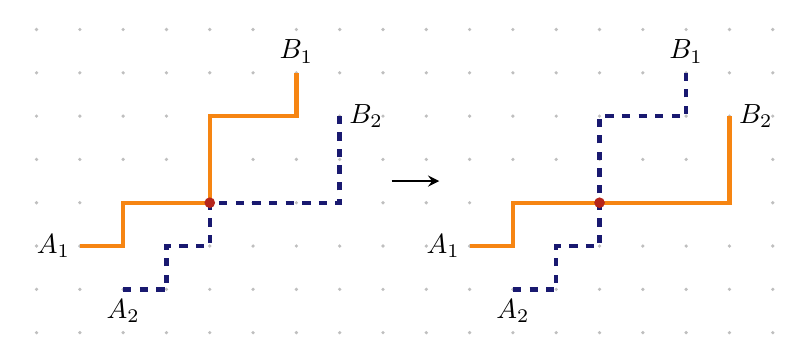
\begin{tikzpicture}[scale=0.55,>=stealth]
\fill[black!25] (-1,-2) circle (1.2pt);
\fill[black!25] (-1,-1) circle (1.2pt);
\fill[black!25] (-1,0) circle (1.2pt);
\fill[black!25] (-1,1) circle (1.2pt);
\fill[black!25] (-1,2) circle (1.2pt);
\fill[black!25] (-1,3) circle (1.2pt);
\fill[black!25] (-1,4) circle (1.2pt);
\fill[black!25] (-1,5) circle (1.2pt);
\fill[black!25] (0,-2) circle (1.2pt);
\fill[black!25] (0,-1) circle (1.2pt);
\fill[black!25] (0,0) circle (1.2pt);
\fill[black!25] (0,1) circle (1.2pt);
\fill[black!25] (0,2) circle (1.2pt);
\fill[black!25] (0,3) circle (1.2pt);
\fill[black!25] (0,4) circle (1.2pt);
\fill[black!25] (0,5) circle (1.2pt);
\fill[black!25] (1,-2) circle (1.2pt);
\fill[black!25] (1,-1) circle (1.2pt);
\fill[black!25] (1,0) circle (1.2pt);
\fill[black!25] (1,1) circle (1.2pt);
\fill[black!25] (1,2) circle (1.2pt);
\fill[black!25] (1,3) circle (1.2pt);
\fill[black!25] (1,4) circle (1.2pt);
\fill[black!25] (1,5) circle (1.2pt);
\fill[black!25] (2,-2) circle (1.2pt);
\fill[black!25] (2,-1) circle (1.2pt);
\fill[black!25] (2,0) circle (1.2pt);
\fill[black!25] (2,1) circle (1.2pt);
\fill[black!25] (2,2) circle (1.2pt);
\fill[black!25] (2,3) circle (1.2pt);
\fill[black!25] (2,4) circle (1.2pt);
\fill[black!25] (2,5) circle (1.2pt);
\fill[black!25] (3,-2) circle (1.2pt);
\fill[black!25] (3,-1) circle (1.2pt);
\fill[black!25] (3,0) circle (1.2pt);
\fill[black!25] (3,1) circle (1.2pt);
\fill[black!25] (3,2) circle (1.2pt);
\fill[black!25] (3,3) circle (1.2pt);
\fill[black!25] (3,4) circle (1.2pt);
\fill[black!25] (3,5) circle (1.2pt);
\fill[black!25] (4,-2) circle (1.2pt);
\fill[black!25] (4,-1) circle (1.2pt);
\fill[black!25] (4,0) circle (1.2pt);
\fill[black!25] (4,1) circle (1.2pt);
\fill[black!25] (4,2) circle (1.2pt);
\fill[black!25] (4,3) circle (1.2pt);
\fill[black!25] (4,4) circle (1.2pt);
\fill[black!25] (4,5) circle (1.2pt);
\fill[black!25] (5,-2) circle (1.2pt);
\fill[black!25] (5,-1) circle (1.2pt);
\fill[black!25] (5,0) circle (1.2pt);
\fill[black!25] (5,1) circle (1.2pt);
\fill[black!25] (5,2) circle (1.2pt);
\fill[black!25] (5,3) circle (1.2pt);
\fill[black!25] (5,4) circle (1.2pt);
\fill[black!25] (5,5) circle (1.2pt);
\fill[black!25] (6,-2) circle (1.2pt);
\fill[black!25] (6,-1) circle (1.2pt);
\fill[black!25] (6,0) circle (1.2pt);
\fill[black!25] (6,1) circle (1.2pt);
\fill[black!25] (6,2) circle (1.2pt);
\fill[black!25] (6,3) circle (1.2pt);
\fill[black!25] (6,4) circle (1.2pt);
\fill[black!25] (6,5) circle (1.2pt);
\fill[black!25] (7,-2) circle (1.2pt);
\fill[black!25] (7,-1) circle (1.2pt);
\fill[black!25] (7,0) circle (1.2pt);
\fill[black!25] (7,1) circle (1.2pt);
\fill[black!25] (7,2) circle (1.2pt);
\fill[black!25] (7,3) circle (1.2pt);
\fill[black!25] (7,4) circle (1.2pt);
\fill[black!25] (7,5) circle (1.2pt);
\draw[BurntOrange,line width=1.6pt] (0,0) -- (1,0) -- (1,1) -- (2,1) -- (3,1) -- (3,2) -- (3,3) -- (4,3) -- (5,3) -- (5,4);
\draw[MidnightBlue,line width=1.6pt,dashed] (1,-1) -- (2,-1) -- (2,0) -- (3,0) -- (3,1) -- (4,1) -- (5,1) -- (6,1) -- (6,2) -- (6,3);
\fill[BrickRed] (3,1) circle (3.5pt);
\node[left] at (0,0) {$A_1$};
\node[below] at (1,-1) {$A_2$};
\fill[black!25] (8,-2) circle (1.2pt);
\fill[black!25] (8,-1) circle (1.2pt);
\fill[black!25] (8,0) circle (1.2pt);
\fill[black!25] (8,1) circle (1.2pt);
\fill[black!25] (8,2) circle (1.2pt);
\fill[black!25] (8,3) circle (1.2pt);
\fill[black!25] (8,4) circle (1.2pt);
\fill[black!25] (8,5) circle (1.2pt);
\fill[black!25] (9,-2) circle (1.2pt);
\fill[black!25] (9,-1) circle (1.2pt);
\fill[black!25] (9,0) circle (1.2pt);
\fill[black!25] (9,1) circle (1.2pt);
\fill[black!25] (9,2) circle (1.2pt);
\fill[black!25] (9,3) circle (1.2pt);
\fill[black!25] (9,4) circle (1.2pt);
\fill[black!25] (9,5) circle (1.2pt);
\fill[black!25] (10,-2) circle (1.2pt);
\fill[black!25] (10,-1) circle (1.2pt);
\fill[black!25] (10,0) circle (1.2pt);
\fill[black!25] (10,1) circle (1.2pt);
\fill[black!25] (10,2) circle (1.2pt);
\fill[black!25] (10,3) circle (1.2pt);
\fill[black!25] (10,4) circle (1.2pt);
\fill[black!25] (10,5) circle (1.2pt);
\fill[black!25] (11,-2) circle (1.2pt);
\fill[black!25] (11,-1) circle (1.2pt);
\fill[black!25] (11,0) circle (1.2pt);
\fill[black!25] (11,1) circle (1.2pt);
\fill[black!25] (11,2) circle (1.2pt);
\fill[black!25] (11,3) circle (1.2pt);
\fill[black!25] (11,4) circle (1.2pt);
\fill[black!25] (11,5) circle (1.2pt);
\fill[black!25] (12,-2) circle (1.2pt);
\fill[black!25] (12,-1) circle (1.2pt);
\fill[black!25] (12,0) circle (1.2pt);
\fill[black!25] (12,1) circle (1.2pt);
\fill[black!25] (12,2) circle (1.2pt);
\fill[black!25] (12,3) circle (1.2pt);
\fill[black!25] (12,4) circle (1.2pt);
\fill[black!25] (12,5) circle (1.2pt);
\fill[black!25] (13,-2) circle (1.2pt);
\fill[black!25] (13,-1) circle (1.2pt);
\fill[black!25] (13,0) circle (1.2pt);
\fill[black!25] (13,1) circle (1.2pt);
\fill[black!25] (13,2) circle (1.2pt);
\fill[black!25] (13,3) circle (1.2pt);
\fill[black!25] (13,4) circle (1.2pt);
\fill[black!25] (13,5) circle (1.2pt);
\fill[black!25] (14,-2) circle (1.2pt);
\fill[black!25] (14,-1) circle (1.2pt);
\fill[black!25] (14,0) circle (1.2pt);
\fill[black!25] (14,1) circle (1.2pt);
\fill[black!25] (14,2) circle (1.2pt);
\fill[black!25] (14,3) circle (1.2pt);
\fill[black!25] (14,4) circle (1.2pt);
\fill[black!25] (14,5) circle (1.2pt);
\fill[black!25] (15,-2) circle (1.2pt);
\fill[black!25] (15,-1) circle (1.2pt);
\fill[black!25] (15,0) circle (1.2pt);
\fill[black!25] (15,1) circle (1.2pt);
\fill[black!25] (15,2) circle (1.2pt);
\fill[black!25] (15,3) circle (1.2pt);
\fill[black!25] (15,4) circle (1.2pt);
\fill[black!25] (15,5) circle (1.2pt);
\fill[black!25] (16,-2) circle (1.2pt);
\fill[black!25] (16,-1) circle (1.2pt);
\fill[black!25] (16,0) circle (1.2pt);
\fill[black!25] (16,1) circle (1.2pt);
\fill[black!25] (16,2) circle (1.2pt);
\fill[black!25] (16,3) circle (1.2pt);
\fill[black!25] (16,4) circle (1.2pt);
\fill[black!25] (16,5) circle (1.2pt);
\draw[BurntOrange,line width=1.6pt] (9,0) -- (10,0) -- (10,1) -- (11,1) -- (12,1) -- (13,1) -- (14,1) -- (15,1) -- (15,2) -- (15,3);
\draw[MidnightBlue,line width=1.6pt,dashed] (10,-1) -- (11,-1) -- (11,0) -- (12,0) -- (12,1) -- (12,2) -- (12,3) -- (13,3) -- (14,3) -- (14,4);
\fill[BrickRed] (12,1) circle (3.5pt);
\node[left] at (9,0) {$A_1$};
\node[below] at (10,-1) {$A_2$};
\node[above] at (5,4) {$B_1$}; \node[right] at (6,3) {$B_2$};
\node[above] at (14,4) {$B_1$}; \node[right] at (15,3) {$B_2$};
\draw[->,thick] (7.2,1.5) -- (8.3,1.5);
\end{tikzpicture}
